%Student_Designed_Experiments
The rest of the course (up to the final) consists of student designed
experiments. The process for the student designed experiments is as follows:

\begin{enumerate}
\item You and your lab group fill out a brainstorming sheet to come up with
possible experiments. You and your lab group prioritize the list and hand it
in.

\item From that list I\ will approve an experiment to try.

\item You will have to write a proposal that describes what you plan to do
for your experiment.

\item Upon approval, you will perform the experiment, and report on the
results in a written paper and a (formal) oral presentation.
\end{enumerate}

We have talked about each of these parts along the way. In this section of
the manual, I\ will describe what I am expecting for each of these
assignments. You will have seen some of this before.

\section{Proposal}

You already have produced a proposal. \ This document was what you used to
convince me that your experiment could work and that you should be given the
resources and support to perform the experiment. Your proposal has the
following parts:

\begin{enumerate}
\item Statement of the experimental problem

\item Procedures and anticipated difficulties

\item Proposed analysis and expected results

\item Preliminary List of equipment needed
\end{enumerate}

We will now reuse these parts to perform the experiment and produce your
final paper and presentation.

\section{Performing the experiment}

I\ will provide you with the equipment we have agreed upon from your
proposal. You will have three lab days to perform your experimentation. I\
will be available for advice and to watch for problems or safety issues. But
you and your team will perform the experiment. You will want to keep good
notes in your lab notebook. You will likely have to change your procedure
after you start because of problems. Take careful note of what was actually
done, and what your measurements were. Note any unusual things that happen.
Carefully record what you do.

\section{Written report}

The written report is designed to match a normal format for an applied
physics article in a journal like\emph{Applied Optics} or the \emph{IEEE
Transactions} journals.\emph{.} There should be an introduction, description
of the procedure, description of the data and results, a description of the
analysis, and a conclusion. These sections are described in detail in the
following table.

\begin{figure}[h!]
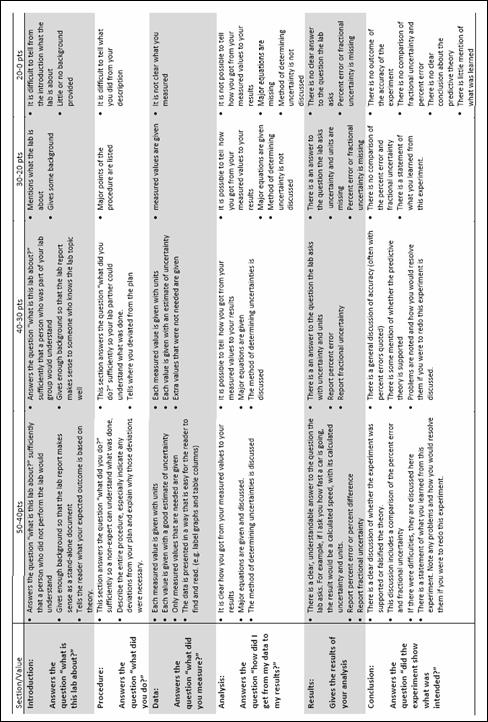
\includegraphics[width=5.2901in,height=7.8049in]{PH4CAX4T}
\end{figure}

\section{Oral report}

Your group will have ten to fifteen minutes to explain your experiment and
present your results and conclusions. I will grade your presentation on the
following areas:

\begin{equation*}
\begin{tabular}{ll}
Professionalism in the delivery & 25 \\ 
Clarity of the delivery & 25 \\ 
Quality of Visual Aids & 25 \\ 
Team support and Participation & 25 \\ 
Total & 100%
\end{tabular}%
\end{equation*}

The format of the presentation should follow the format of the written
report. Don't forget to give proper credit for pictures, or ideas and
quotations in your presentation just as you will in your written report.

\section{Lab Notebook}

Hopefully you noticed that a lab notebook is required for this class. The
lab notebook is designed to be a record of what you did. If you had to
repeat today's experiment five years from now, could you do it based on what
you write today?

At most professional labs and major engineering companies your lab notebook
is considered the property of the company or organization. It is the proof
that you did the experiment that you say you did, and that you got the
results you say you got. It has to be readable and understandable to someone
who did not participate in the lab with you. This is a pretty tall order.

Of course the evidence that you participated in the group project will all
be found in your lab notebook. You have had experience in PH150 and
throughout PH250. So you are an expert in keeping lab notebooks. But as
usual with a group project not all of what happens will be written in your
notebook. Some will be in your coworker's notebooks. That is fine, because
you know to refer to that work in your notebook with a reference to the
notebook of the person that did the work. Note that the grade for the lab
notebook is a {\Large large} part of your semester grade, this represents
the fact that your lab notebook is a {\Large large} part of what a scientist
does. Remember that the lab notebook must be kept \emph{as you go}. It is
not OK to try to recreate it after the experiment is over. This takes time
away from fiddling with equipment and thinking about procedure, but it 
\textsc{is part of performing the experiment.} So recreating something at
the end is the same as not doing the assignment. When you are practicing in
your field you will find that courts of law feel the same way about lab
notebooks. To prove you own the intellectual property you have developed,
the lab notebook has to be kept \emph{as you go}.

Here are reminders from PH150 on how to keep a lab notebook:

\subsection{Designing the Experiment}

In PH150 we learned that to design an experiment we needed the following
steps. Some evidence of these steps should be found in your lab notebook:

\begin{enumerate}
\item Identify the system to be examined. Identify the inputs and outputs.
Describe your system in your lab notebook.

\item Identify the model to be tested. Express the model in terms of an
equation representing a prediction of the measurement you will make. Record
this in your lab notebook. (If you have not solved this problem in your
PH121 class yet, call me over and we will go through it together).

\item Plan how you will know if you are successful in your experiment. Plan
graphs or other reporting devices. Record this in your lab notebook.

\item Rectify your equation if needed. Record this in your lab notebook.

\item Choose ranges of the variables. Record this in your lab notebook.

\item Plan the experimental procedure. Record this in your lab notebook.

\item Perform the experiment . Record this in your lab notebook (see next
section). You will need your uncertainty equations from the proposal.
\end{enumerate}

\subsection{Performing the Experiment}

Step 8 is really many individual steps recording the actual performance of
the experiment. You learned this in PH150, but here is a review of the
criteria I\ will use to grade your lab book:

\begin{itemize}
\item Describing the goal for the work

\begin{itemize}
\item Usually this takes the form of a physical law we will test.
\end{itemize}

\item Give predictive equations and uncertainties for the predictions based
on the physical law.

\begin{itemize}
\item This usually involves forming a mathematical model. You should record
any assumptions that went into the model (e.g. no air resistance, point
sources, massless ropes, etc.).
\end{itemize}

\item Give your procedure

\begin{itemize}
\item Recording what you really did (not the lab instructions), tell what
changes you make in your procedure as you make them.

\item Record as you do the work.

\item Record the equipment used and settings, values, etc. for that
equipment (see next item).

\item Did you learn how to use any new equipment? What did you learn that
you want to recall later (say, when taking the final, or when you are a
professional and need to use a similar piece of equipment five years from
now).
\end{itemize}

\item Record the data you used. . The data are all the measurements you took
plus your best estimate of the uncertainties in the measurements. Record any
values you got from tables or published sources (or from your professor) and
state where you got these values. You don't always want to write down all
the data you use. If you have a large set of values, you can place them in a
file, and then record the file name and location in your lab notebook. Make
sure this is a file location that does not change (emailing the data to
yourself is not a good plan).

\item Give a record of the analysis you performed. You should have given
some idea of how you got your predictive equation. Now, what did you do to
get the data through the equation? Were there any extra calculations? Did
you obtain a set of \textquotedblleft truth data\textquotedblright\ (data
from tables or published sources, or from an alternate experiment) for your
experiment? If so, did you do any calculations, have any uncertainty, etc.
associated with the truth values?

\item Give a brief statement of your results and their associated
uncertainties.

\item Draw conclusions

\begin{itemize}
\item Do your results support the theory? Why or why not? What else did you
learn along the way that you want to record.

\item This is where we may compare the percent error to our relative
uncertainty.
\end{itemize}
\end{itemize}

This may seem like a lot of work (that is because it IS a lot of work). It
takes practice to be able to do this professionally, which is why we do it
here.
